\documentclass[12pt]{article}
\usepackage{amsmath}
\usepackage{amssymb}
\usepackage{geometry}
\usepackage{amsmath, amsfonts, bm, graphicx}
\usepackage{tabularx}
\usepackage{booktabs} 
\usepackage{float}
\usepackage{wrapfig}
\geometry{margin=1in}
\title{}
\date{}
\author{}

\begin{document}

\textbf{SI Prefixes}
\[\begin{aligned}
\text{femto (f)}  &= 10^{-15} \\
\text{pico (p)}   &= 10^{-12} \\
\text{nano (n)}   &= 10^{-9} \\
\text{micro ($\mu$)}  &= 10^{-6} \\
\text{milli (m)}  &= 10^{-3} \\
\text{centi (c)}  &= 10^{-2} \\
\text{deci (d)}   &= 10^{-1} \\
\text{deca (da)}  &= 10^{1} \\
\text{hecto (h)}  &= 10^{2} \\
\text{kilo (k)}   &= 10^{3} \\
\text{mega (M)}   &= 10^{6} \\
\text{giga (G)}   &= 10^{9} \\
\text{tera (T)}   &= 10^{12} \\
\text{peta (P)}   &= 10^{15} \\
\end{aligned}\]
\underline{Note:} $1\text{Angstrom}\,(\text{\AA}) = 10^{-10}$ m
\newpage
\section*{\LARGE\underline{Mechanical Properties}}
\section*{Stress and Strain}
\textbf{Types of loading}
\begin{figure}[H]
    \centering
    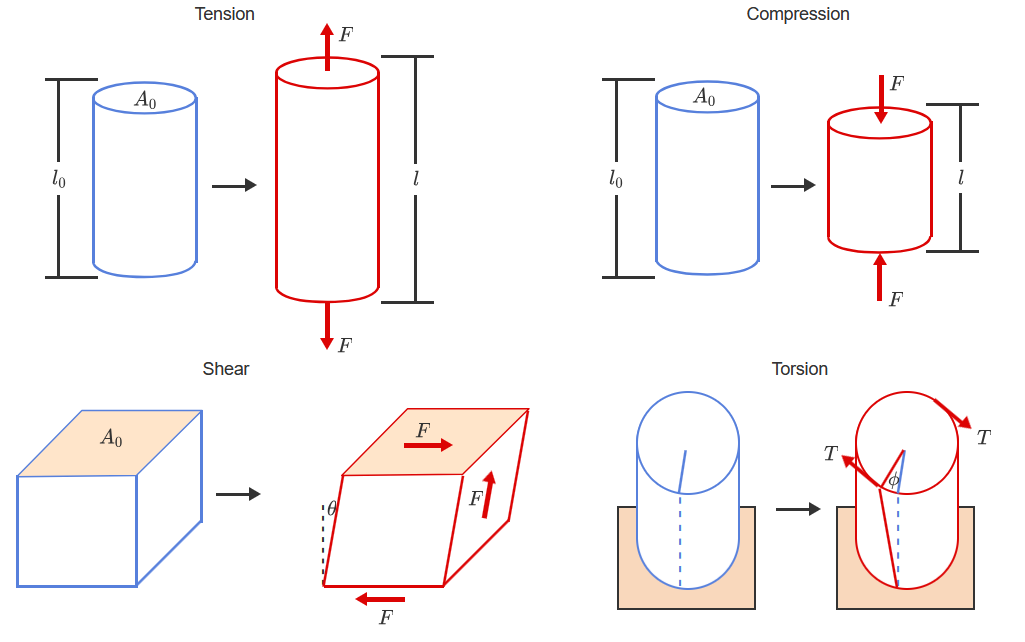
\includegraphics[width=0.8\textwidth]{types of loading.png}
\end{figure}
\newpage
\noindent \textbf{Stress (Force Normalized by Area)}\\\\
Tensile and Compression Stress
\[\sigma = \frac{F}{A_o} \quad \text{(in units of pressure)}\]
Shear Stress
\[\tau = \frac{F}{A_o}\]
\noindent \textbf{Strain (Displacement Normalized by Original Length)}\\\\
Tensile and Compression Strain
\[\epsilon = \frac{l - l_0}{l_0}\]
Shear Strain
\[\gamma = \tan\theta \quad \text{($\theta$ is the shear angle)}\]

\noindent \textbf{Normal and Shear Stress Along an Angled Plane}
\begin{figure}[H]
    \centering
    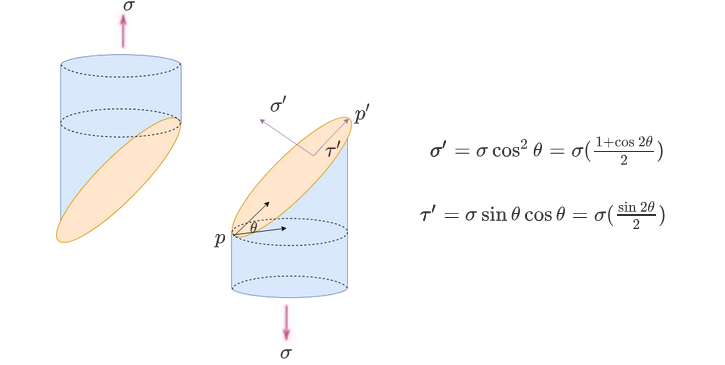
\includegraphics[width=0.8\textwidth]{geometric stress.png}
\end{figure}
\newpage

\section*{Elastic Deformation}
\textbf{Relationship Between Stress and Strain}\\\\
Tensile and Compression
\[\sigma = E\epsilon \quad \text{(E (GPa or psi) is the modulus of elasticity)}\]
Shear
\[\tau = G\gamma \quad \text{(G is the shear modulus)}\]
\underline{Note:} The modulus of elasticity (Young's modulus) is the slope of the stress - strain plot. (It describes a material's resistance to elastic deformation. Stiffer $\implies$ higher E)\\\\
\textbf{Anelasticity:} time dependent elastic strain, where deformation and recovery is not instantaneous.\\
\textbf{Viscoelastic behavior}: materials (such as polymers) with significant anelasticity\\\\

\noindent \textbf{Poisson's Ratio}
\begin{figure}[H]
    \centering
    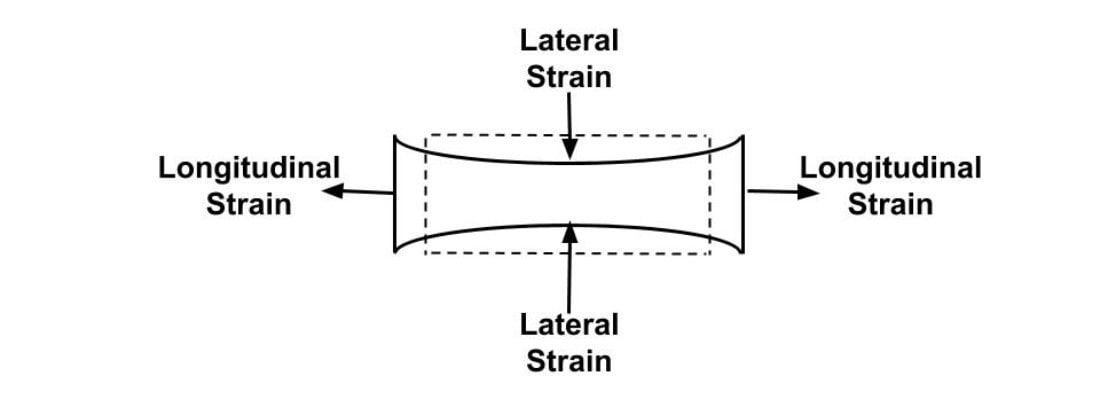
\includegraphics[width=0.8\textwidth]{poissons.jpg}
\end{figure}
\[ \nu = -\frac{\epsilon_{\text{lateral}}}{\epsilon_{\text{longitudinal}}}\]
\underline{Note:} Lateral is perpendicular to the direction of loading and longitudinal is along the direction of loading
\newpage
\underline{Example:} Rectangular prism
\begin{figure}[H]
    \centering
    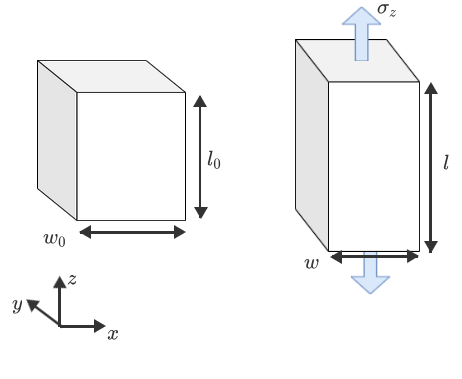
\includegraphics[width=0.4\textwidth]{poissons 2.png}
\end{figure}
\noindent If the applied stress is uniaxial (only along 1 axis) and the material is isotropic (constant properties regardless of direction), then for a $\sigma_z$, $\epsilon_x=\epsilon_y$
\[ \nu = -\frac{\epsilon_x}{\epsilon_z}= -\frac{\epsilon_y}{\epsilon_z}\]

\noindent \textbf{Relating modulus of elasticity, shear modulus and Poisson's ratio}
\[E=2G(1+\nu)\]
\underline{Note:} Some materials (like foams) expand under tension so they have a negative Poisson's ratio, these materials are called \textbf{auxetics}.
\newpage
\section*{Plastic Deformation}
\begin{wrapfigure}{l}{0.4\textwidth}
    \centering
    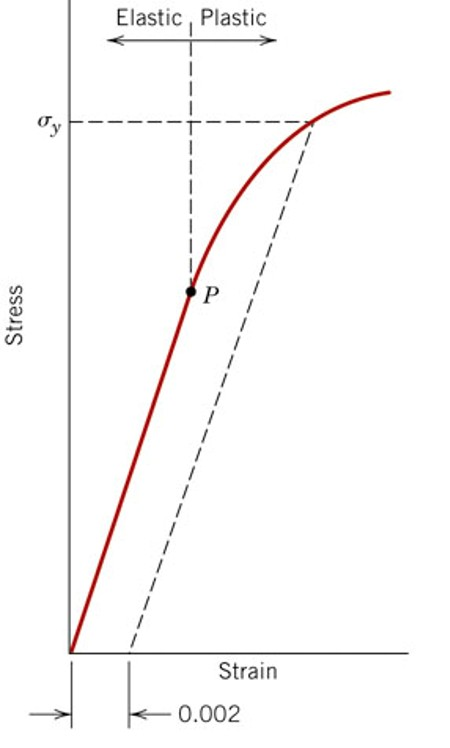
\includegraphics[width=0.4\textwidth]{yield.jpg}
\end{wrapfigure}
Point P is the \textbf{Proportional Limit} where the exact departure from linearity occurs and deformation becomes permanent.
\\\\
\textbf{Yield Stress ($\sigma_y$):} stress at which noticeable strain has occurred (0.002)
\\\\\\\\\\\\\\\\\\\\\\\\\\\\\\\\\\\\\\
\begin{figure}[H]
    \centering
    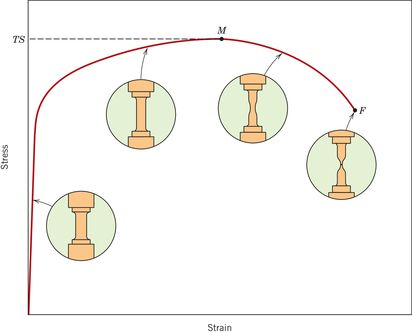
\includegraphics[width=0.55\textwidth]{tensile.jpg}
\end{figure}
\noindent\textbf{Tensile Strength}: Stress at the maximum point on the stress - strain plot. After this point, necking occurs and all deformation is focused at the neck until fracture (point F)

\noindent\textbf{Ductility}\\\\
As $\%$ elongation:
\[\%EL = \frac{l_f - l_0}{l_0} \times 100\]
As $\%$ reduction in area
\[\%RA = \frac{A_0 - A_f}{A_0} \times 100\]
$l_f$ and $A_f$ are length and cross sectional area of sample at fracture respectively.\\\\
\noindent\textbf{Resilience:} capacity of a material to absorb energy when it is deformed elastically and unloaded (similar to spring potential energy)\\\\
\noindent\textbf{Modulus of Resilience}
\[U_r = \int_{0}^{\epsilon_{yield}}\sigma d\epsilon\]
Area under the stress - strain plot from 0 to yield point\\\\
Assuming a linear elastic region:
\[U_r=\frac{1}{2}\sigma_y\epsilon_y\]
\newpage
\section*{\LARGE\underline{Crystal Structures}}
\noindent\textbf{Atomic Packing Factor}
\[ APF = \frac{\text{Volume of atoms in unit cell}}{\text{Total unit cell volume}}\]
\noindent\textbf{Packing Fraction}
\[PF=\frac{\text{Total Cross Sectional Area of Atoms}}{\text{Total Area of Plane}}\]
\noindent\textbf{Number of Atoms per Unit Cell}
\[N=N_i+\frac{N_f}{2}+\frac{N_c}{8}\]
$N_i$ are interior atoms, $N_f$ are face atoms and $N_c$ are corner atoms
\section*{Simple Cubic}
\begin{figure}[H]
    \centering
    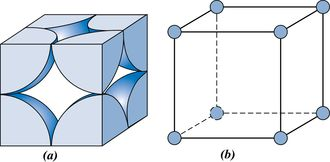
\includegraphics[width=0.6\textwidth]{SC.jpg}
\end{figure}
\[2R=a\]
\[APF=\frac{(\text{\# atoms})(\text{volume/atom})}{(\text{volume/unit cell})}\]
\[APF=\frac{(1)(\frac{4}{3}\pi(a/2)^3)}{a^3}\]
\section*{Body Centered Cubic}
\begin{figure}[H]
    \centering
    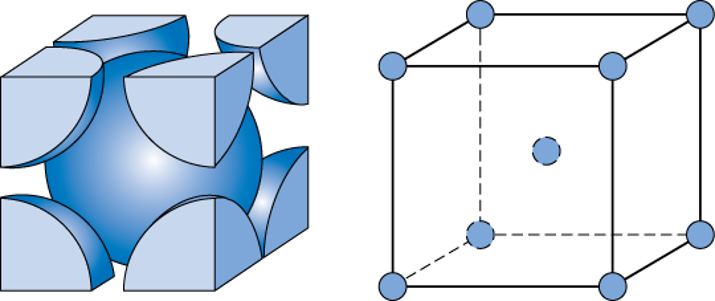
\includegraphics[width=0.6\textwidth]{BCC.png}
\end{figure}
\[\text{Triangle formed along the main diagonal and face diagonal}\]
\begin{figure}[H]
    \centering
    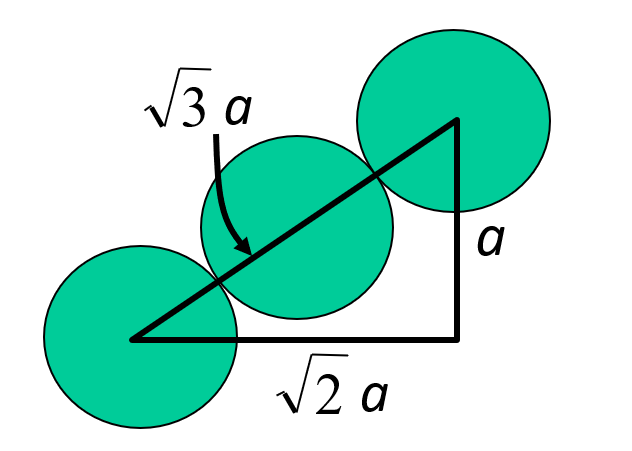
\includegraphics[width=0.3\textwidth]{BCC diag.png}
\end{figure}
\[4R=\sqrt{3}a\]
\[APF=\frac{(\text{\# atoms})(\text{volume/atom})}{(\text{volume/unit cell})}\]
\[APF=\frac{(2)(\frac{4}{3}\pi(\sqrt{3}/4a )^3)}{a^3}\]
\newpage

\section*{Face Centered Cubic}
\begin{figure}[H]
    \centering
    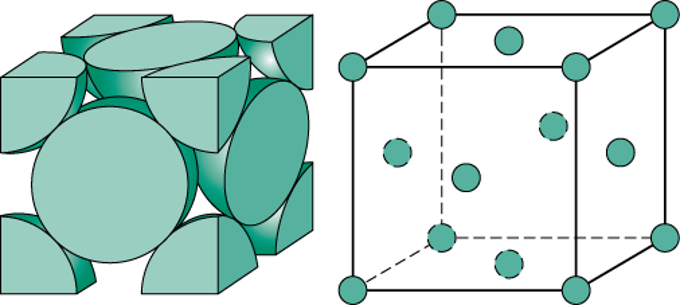
\includegraphics[width=0.6\textwidth]{FCC.png}
\end{figure}
Along the face diagonal:
\[4R=\sqrt{2}a\]
\[APF=\frac{(\text{\# atoms})(\text{volume/atom})}{(\text{volume/unit cell})}\]
\[APF=\frac{(4)(\frac{4}{3}\pi(\sqrt{2}/4a )^3)}{a^3}\]
\newpage
\section*{Hexagonal Close Packed}
\begin{figure}[H]
    \centering
    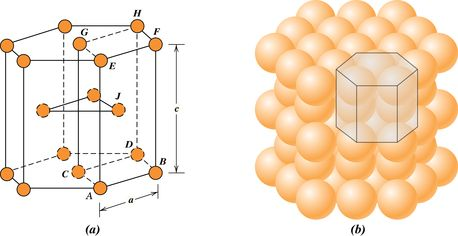
\includegraphics[width=0.6\textwidth]{HCP.jpg}
\end{figure}
\begin{figure}[H]
    \centering
    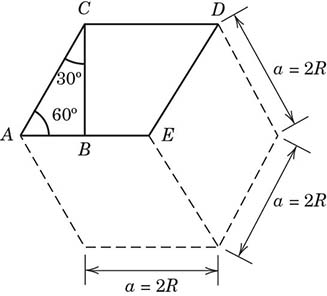
\includegraphics[width=0.4\textwidth]{Untitled.jpg}
\end{figure}
Area of base hexagon is 3 parallelograms or 6 equilateral triangles:
\[\text{Area}=\frac{3a^2\sqrt{3}}{2}\]
Given height c:
\[\text{Volume of unit cell}=\frac{3a^3\sqrt{3}}{2}\]
\newpage
\section*{Theoretical Density for Crystals}
\[\rho=\frac{(\text{atoms/unit cell})(\text{g/mol})}{(\text{vol/unit cell})(\text{atoms/mol})}=(\text{g/vol})\]
\[\rho=\frac{nA}{V_c N_A}\]
Where:
\begin{itemize}
    \item n = \# of atoms in unit cell
    \item A = atomic weight
    \item $V_c$ = volume of unit cell
    \item $N_a$ = Avogadro's number ($6.022 \times 10^{23 }\text{ atoms/mol}$)
\end{itemize}
\section*{Ceramic Crystal Structures}
Factors that determine crystal structure:
\begin{itemize}
    \item Relative sizes of ions ($\frac{r_{cation}}{r_{anion}}$)
    \item Maintenance of charge neutrality (Net charge in ceramic is zero)
\end{itemize}
\underline{Note:} As $\frac{r_{cation}}{r_{anion}}$ increases, so does coordination number
\begin{figure}[H]
    \centering
    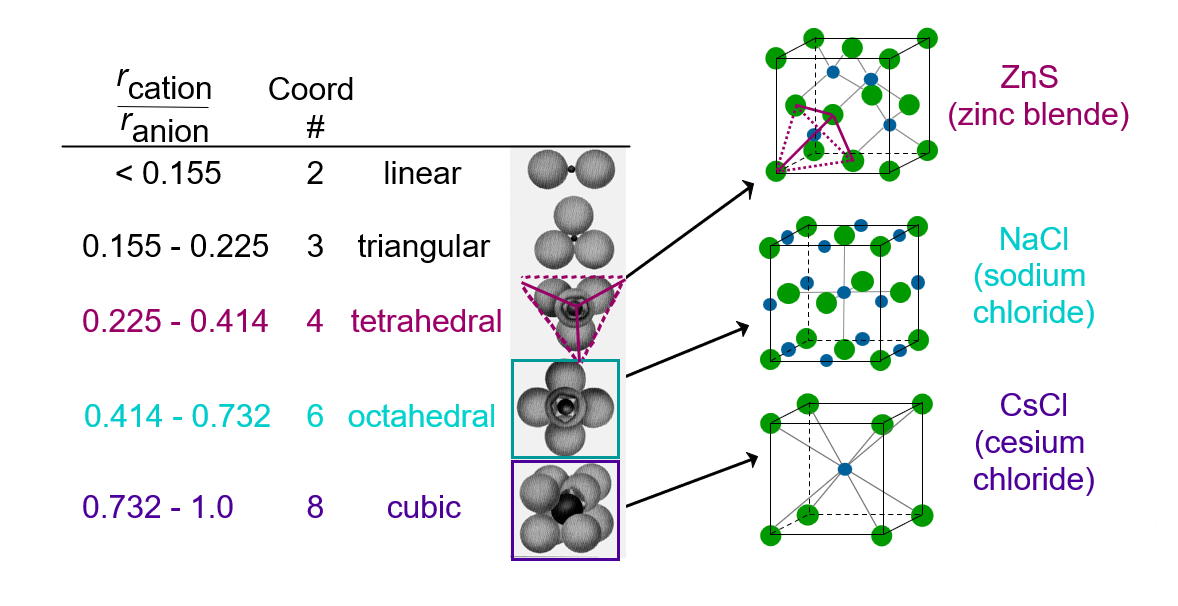
\includegraphics[width=0.8\textwidth]{ceramic.png}
\end{figure}
\newpage
\noindent\textbf{Theoretical Density for Ceramics}
\[\rho =\frac{n'(\sum A_C+\sum A_A)}{V_c N_A}\]
Where:
\begin{itemize}
    \item n' = \# of Atoms per unit cell (For AX structures, this is equal for cations and anions)
    \item $\sum A_A$ = sum of cation molar mass
    \item $\sum A_C$ = sum of anion molar mass
    \item $V_c$ = volume of unit cell
    \item $N_A$ = Avogadro's number ($6.022 \times 10^{23} \text{ atoms/mol}$)
\end{itemize}
\section*{Rock Salt Structure}
\begin{figure}[H]
    \centering
    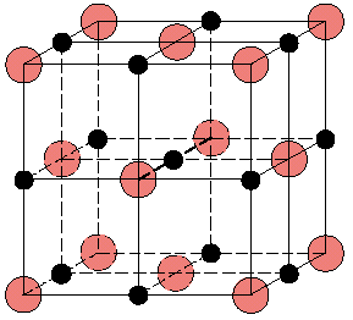
\includegraphics[width=0.4\textwidth]{Rocksalt.png}
\end{figure}
\underline{Note:} Cations prefer octahedral sites (in black)\\
Along the edges:
\[2R_A+2R_C=a\]
\section*{AX Crystal Structure (Cesium Chloride)}
\begin{figure}[H]
    \centering
    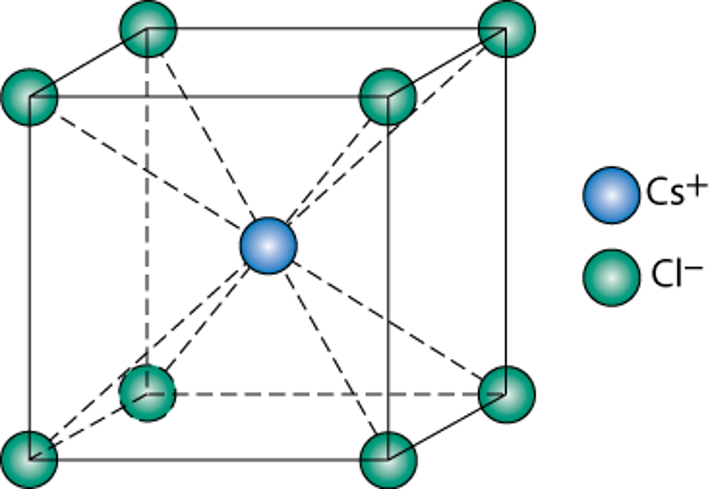
\includegraphics[width=0.4\textwidth]{AX.png}
\end{figure}
\underline{Note:} Cations prefer cubic sites (Body Center, in blue) \\
Across the main diagonal:
\[2R_A+2R_C=\sqrt{3}a\]
\section*{AX$_2$ Crystal Structures (Flourite)}
\begin{figure}[H]
    \centering
    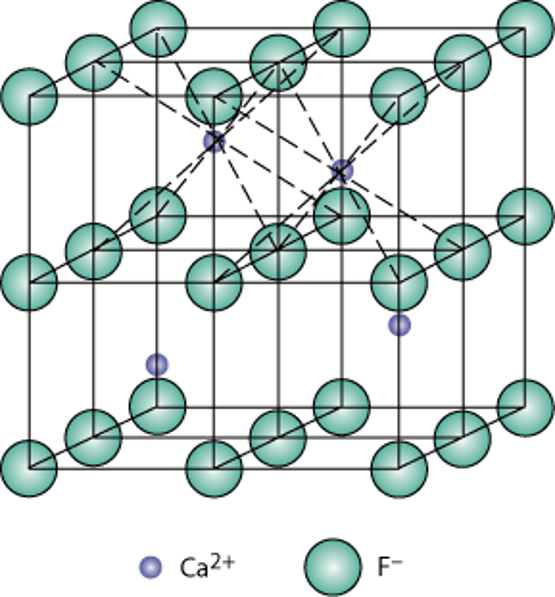
\includegraphics[width=0.4\textwidth]{AX2.png}
\end{figure}
\underline{Note:} Cations prefer cubic sites (Body Center, in blue) \\
There are half as many Ca$^{2+}$ as F$^-$ (for CaF$_2$)
\section*{ABX$_3$ Crystal Structure (Perovskite)}
\begin{figure}[H]
    \centering
    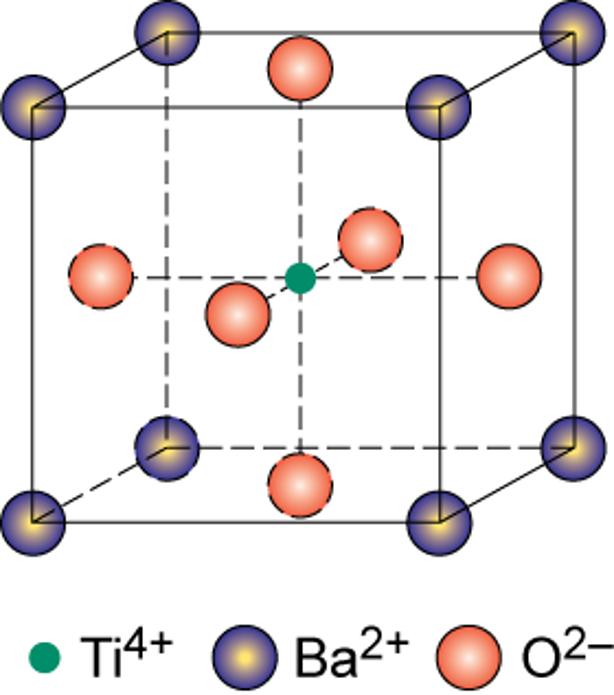
\includegraphics[width=0.4\textwidth]{ABX3.png}
\end{figure}
\section*{Point Coordinates}
To find the coordinate indices (q,r,s), find the cartesian coordinates and divide by the corresponding lattice parameter
\[(q,r,s) = \left( \frac{x}{a}, \frac{y}{b}, \frac{z}{c} \right)\]
\section*{Crystallographic Directions}
How to define:
\begin{itemize}
    \item Position vector to pass through origin
    \item Read off projections onto coordinate axes in terms of lattice parameters (a,b,c)
    \item Multiply through by common denominator
    \item Enclose in square brackets without commas, negatives go on top (ex: [$\overline{1} 2 3$])
\end{itemize}
How to read [123]:
\begin{itemize}
    \item Divide by the common denominator used previously (say 6)
    \item Vector in cartesian: (1/6,1/3,1/2)
\end{itemize}
\section*{Crystallographic Planes}
How to define with Miller indices:
\begin{itemize}
    \item Define any origin
    \item Read intercepts of the plane with the coordinate axes in terms of lattice parameters (a,b,c)
    \item Take reciprocals of intercepts
    \item Enclose in parenthesis without commas, negatives go on top (ex: ($\overline{1} 2 3$))
\end{itemize}
How to read:
\begin{itemize}
    \item Take reciprocols of plane to identify intercepts
\end{itemize}
\section*{Linear and Planer Density}
\textbf{Linear Density}
\[LD = \frac{\text{Number of atom centered on line}}{\text{Unit length of direction vector}}\]
\textbf{Planer Density}
\[PD=\frac{\text{Number of atoms centered on plane}}{\text{Area of plane}}\]
\newpage
\section*{\LARGE\underline{Dislocations and Strengthening Mechanisms}}
\section*{Basic Concepts}
\textbf{Types of dislocations}
\end{document}